\documentclass[border=2pt]{standalone}
\usepackage{tikz}
\usetikzlibrary{automata,arrows.meta}
\begin{document}
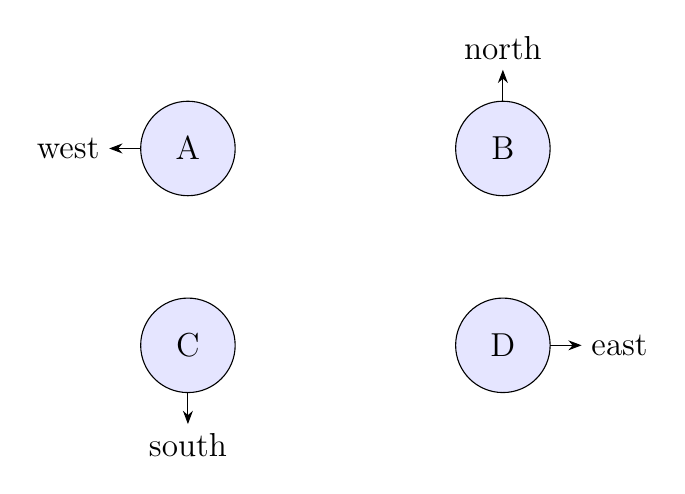
\begin{tikzpicture}[>=Stealth,font=\large,every state/.style={fill=blue!10,minimum size=12mm,outer sep=0pt},accepting distance=4mm]
  \node[state,accepting by arrow,accepting where=left,accepting text=west] (A) at (0,0) {A};
  \node[state,accepting above,accepting text=north] (B) at (4,0) {B};
  \node[state,accepting below,accepting text=south] (C) at (0,-2.5) {C};
  \node[state,accepting right,accepting text=east] (D) at (4,-2.5) {D};
\end{tikzpicture}
\end{document}
